% proposal skripsi.
\documentclass{jtetiproposalskripsi}

%-----------------------------------------------------------------
%Disini awal masukan untuk data proposal skripsi
%-----------------------------------------------------------------
\titleind{SISTEM PENGAMAN RUMAH BERBASIS GPRS DAN IMAGE CAPTURING DENGAN MENGUNAKAN BAHASA PEMPROGRAMAN VISUAL BASIC 6.0}

\fullname{AHMAD MURSYID}

\idnum{1110652016}

\approvaldate{06 Januari 2015}

\degree{Sarjana Teknik Informatika}

\yearsubmit{2015}

\program{Teknik Informatika}

\headprogram{mursyid}

\dept{Teknologi Informasi}

\firstsupervisor{Taufiq Timur W. S.Kom., M.Kom}
\firstnip{1976 0501 2002 12 1 002}

\secondsupervisor{Triawan Adi Cahyanto}
\secondnip{1977 0131 2002 12 1 003}


%-----------------------------------------------------------------
%Disini akhir masukan untuk data proposal skripsi
%-----------------------------------------------------------------

\begin{document}

\cover

\approvalpage

%-----------------------------------------------------------------
%Disini akhir masukan untuk muka skripsi
%-----------------------------------------------------------------

%-----------------------------------------------------------------
%Disini awal masukan Intisari
%-----------------------------------------------------------------
\begin{abstractind}
Alat ini dibuat untuk memudahkan kita untuk mengontrol keamanan rumah apabila ditinggal dalam keadaan kosong media yang digunakan adalah Handphone, dengan memanfaatkan fasilitas MMS dan GPRS.
             Alat ini terdiri dari satu kamera webcam, empat sensor yaitu satu sensor Suhu sebagai pengontrol suhu temperatur di dalam rumah, satu sensor PIR (Passive Infra Red) sebagai pendeteksi gerak gerik manusia yang ada di sekitarnya, tiga sensor Infra red untuk pintu depan, pintu belakang dan jendela, dan satu sensor Ultrasonik, jadi sensor PIR dan kamera webcam ditempatkan didepan rumah, apabila ada gerakan, maka sensor PIR akan mendeteksi gerakan tersebut dan selanjutnya mikro akan mengirim SMS dua kali melalui HP stasioner SMS yang pertama untuk pemberitahuan ke HP tujuan yang berupa teks “intruders” dan SMS yang kedua dikirim ke kamera digital berupa teks juga, yang mana pengiriman SMS ini sebagai pemberitahuan ke kamera untuk mengambil gambar situasi keadaan setelah kamera mengambil gambar, kemudian gambar tersebut akan dikirim ke HP tujuan melalui media MMS. 
             Kamera digital ini mempunyai sim-card di dalamnya sebagai sarana untuk mengirim SMS dan MMS. Kemudian untuk sensor switch ditaruh di dekat pintu dan jendela, jadi apabila pintu dan jendela kebuka maka mikro akan mengirim SMS ke HP tujuan yang berupa teks pemberitahuan yaitu “intruders”.
              Mikrokontroler AT89S8252 sebagai basis pengontrolnya. Kemudian alat ini juga dapat mengambil gambar situasi setiap saat dengan meggunakan fasilitas SMS, yaitu dengan cara kita mengirim SMS ke kamera digital yang berupa teks yaitu (1)(spasi)(no hp tujuan). 
             Alat Pengendali keamanan berbasis Mikrokontroler ini akan bekerja sesuai dengan program yang ada. Kemudian Mikrokontroler akan mengirimkan SMS untuk memberikan status situasi. Dalam tugas akhir ini  yang dibahas yaitu  sistem keamanan rumah dengan fasilitas SMS dan MMS serta pengukuran alat dan pengujian alat.
            Alat yang dirancang ini memiliki tiga sensor, satu buah mikrokontroler, dan satu buah kamera digital.


 


\bigskip
\textbf{Kata kunci} : \emph{mikrokontroler}
\end{abstractind}
%-----------------------------------------------------------------
%Disini akhir masukan Intisari
%-----------------------------------------------------------------

\tableofcontents
\addcontentsline{toc}{chapter}{DAFTAR ISI}
\selectlanguage{bahasa}\clearpage\pagenumbering{arabic}\setcounter{page}{1}

%-----------------------------------------------------------------
%Disini awal masukan untuk Bab
%-----------------------------------------------------------------
\chapter{LATAR BELAKANG}

\section{Latar Belakang Masalah}
Perkembangan teknologi komunikasi saat ini berkembang sangat pesat, salah satunya adalah handphone. Dengan alat ini kita dapat berkomunikasi jarak jauh dengan mudah dan alat ini dapat dibawa kemana saja, karena bentuk dan ukurannya yang kecil. Selain itu, handphone juga memiliki beragam fasilitas, seperti, Short Message Service (SMS), Multimedia Message Service (MMS), General Packet Radio Service (GPRS), Kamera, Ringtones,  dan lain sebagainya.
Dalam dunia Information Technology (IT) segala upaya dilakukan dengan membuat berbagai macam eksperimen, guna membuat suatu sistem yang baru dan semakin mempermudah kerja sistem tersebut. Diantaranya ada suatu sistem pengendali terhadap suatu peralatan yang berkembang saat ini. Sistem pengendali peralatan yang berkembang saat ini  adalah sistem untuk rumah tangga, perkantoran dan perkuliahan.
Seiring dengan perkembangan ilmu pengetahuan dan teknologi (IPTEK) terutama dalam teknologi komputerisasi dan komunikasi, telah banyak penemuan sistem-sistem komputer yang memanfaatkan media komunikasi, yaitu memanfaatkan fasilitas handphone, yang bertujuan guna memberikan kemudahan dalam hal pekerjaan, pengembangan dari sistem pengaman rumah berbasis sms (Dhanis Firdaus 2006), (Susanto Wibisono Koselan, maret 2001, www.mikroelektronika.co.yu).
Melihat perkembangan teknologi tersebut, tentunya teknologi komputer dan media komunikasi ini dapat kita gunakan dalam pengembangan sistem pengaman rumah, diharapkan sistem pengaman rumah yang berbasis GPRS ini dapat lebih terjamin lagi keamanannya, karena dalam sistem pengaman rumah yang ada sekarang ini, masih belum dapat memberikan jaminan keamanan bagi rumah kita, walaupun di dalam rumah kita telah terpasang sistem pengaman rumah, terkadang kita sering curiga akan keamanan rumah kita bila kita tinggal dalam keadaan kosong sampai berhari-hari, karena dalam proses kerja sistem ini, kita harus selalu berada dalam lingkungan rumah. 
Dengan menimbang permasalahan diatas, maka sistem komputer juga dapat kita jadikan sebagai pengontrol pengaman rumah, dengan memanfaatkan fasilitas handphone yaitu fasilitas General Packet Radio Service (GPRS) dan Image Capturing, tentunya sistem pengaman rumah akan lebih terjamin lagi keamanannya, karena kita bisa mengontrol keadaan rumah tanpa harus selalu ada di dalam rumah, kita dapat memonitor keamanan rumah melalui handphone setiap kemungkinan kondisi bahaya yang terjadi.
Untuk mengontrol sistem pengaman rumah ini di perlukan suatu perangkat lunak yang di gunakan untuk mengatur nomor handphone sebagai penerima pesan, selain itu juga berfungsi sebagai display (tampilan) suhu dalam rumah, dan dengan memanfaatkan Image Capturing kita dapat mengaplikasikan gambar tersebut kedalam komputer, saluran Port Serial (DB9) dan USB sebagai interface antara (software) dan rangkaian (hardware).



\section{Tujuan Penelitian}
Tugas akhir ini bertujuan membuat sebuah alat yang menggunakan fasilitas yang ada pada handphone yaitu Multimedia Message Service (MMS) dan General Packet Radio Service (GPRS) agar dapat memonitor keamanan rumah melalui handphone. Fasilitas tersebut sebetulnya sebuah perintah kepada mikrokontroller untuk mengontrol keamanan rumah kita, kemudian alat ini akan mengirim gambar apabila sensor terpicu dengan gerakan, maka kamera akan memotret dan mengirimkan gambar situasi ke sebuah nomor lain. Dan alat ini juga dapat mengontrol situasi keamanan rumah kita setiap saat.


\section{Manfaat Penelitian}
Manfaat yang ingin di capai penulis dalam pembuatan sistem ini adalah :
1.Menjadikan sistem pengaman rumah lebih terjamin lagi keamanannya, efisien dan lebih otomatis. 
2.Mengembangkan sistem pengaman rumah yang telah ada saat ini.
3.Meningkatkan kreatifitas berfikir mahasiswa dalam mengembangkan penggunaan komputer untuk pengaplikasiannya.
4.Memberikan sumbangan bagi perkembangan ilmu pengetahuan khususnya dalam bidang Information Technology (IT).
%-------------------------------------------------------------------------------
\chapter{TINJAUAN PUSTAKA DAN DASAR TEORI}                

\section{Handphone}
Handphone (telepon genggam) atau yang sering disebut Telepon Selular merupakan alat komunikasi dengan teknologi yang lebih tinggi dibandingkan dengan telepon rumah PSTN (Public Switch Telephone Network), karena pada handphone banyak terdapat fasilitas-fasilitas (fitur) yang tidak terdapat pada PSTN seperti, SMS (Short Message Service), MMS (Multimedia Message Service), GPRS (General Packet Radio Service), Ringtone, Radio, Kamera dan lain sebagainya. Teknologi yang digunakan sistem seluler sendiri beragam, ada AMPS, GSM, dan CDMA. Tapi, apa pun teknologinya, mereka termasuk keluarga telepon seluler. Sistem ini menyediakan komunikasi wireless bagi pelanggan (yang berlokasi dalam jangkauan radio sistem) untuk berhubungan dengan pelanggan seluler lain atau dengan pelanggan PSTN (di Indonesia, dipegang PT Telkom). Saat ini, sistem telepon seluler menyediakan layanan lebih banyak, dibanding sistem telepon kabel.


\section{Port serial}
Dalam serial interface, RS 232 memanfaatkan sebuah konektor dengan jumlah pin sebanyak 9. Konektor ini sering di sebut DB9 Connector. Konektor DB9 dalam sistem ini berfungsi untuk menghubungkan antara rangkaian pengontrol elektronik dengan handshet (Handphone).

\section{2.4.Mikrokontroler AT89S8253}
Mikrokontroler tipe AT89S8253 merupakan pengembangan dari mikrokontroler tipe standard MCS-51 (8031,8751,8051). Hal yang terdapat pada penjelasan mikrokontroler tipe MCS-51 juga berlaku untuk mikrokontroler tipe AT89S8253. Karena adanya tambahan fitur yang tidak terdapat pada mikrokontroler tipe MCS-51, maka mikrokontroler tipe AT89S8253 dapat menggantikan mikrokontroler tipe MCS-51, tetapi tidak demikian sebaliknya.
Berikut ini adalah fitur-fitur untuk mikrokontroler tipe AT-89S8253 produksi ATMEL.





%-------------------------------------------------------------------------------
\chapter{METODOLOGI}

\section{Alat dan Bahan}
Bahan yang digunakan dalam penelitian ini adalah:

\vspace{-0.5cm}

\begin{enumerate}[a.]
\begin{singlespace}
\itemsep0em
\item Komputer minimal Pentium II,
\item Kabel Data Handphone,
\item Handphone Sony Ericson W550i
\item Kabel  Saluran Port Serial (DB9) 
\item Rangkaian Sistem Pengaman Rumah
\end{singlespace}
\end{enumerate}

\section{Langkah Kerja}
Rancangan arsitektur yang akan digunakan pada penelitian ini 

\textbf{WP 1: Perancangan Perangkat Lunak}

Dalam kegiatan tugas akhir ini, memerlukan beberapa perangkat untuk mendukung dalam proses pengerjaanya, ada beberapa perangkat yang dibutuhkan antara lain perangkat keras dan perangkat lunak.
Sistem Operasi Microsoft Windows XP, Bahasa Pemrograman Microsoft Visual Basic 6.0


\textbf{WP 2: Implementasi Perangkat Lunak}

Implementasi perangkat lunak dilakukan pada tahap ini. Langkah pertama yang dilakukan adalah memastikan bahwa rangkaian dapat terhubungan dengan yang direncanakan.

\textbf{WP 3: Integrasi dan Pengujian Seluruh Sistem}

Dalam kerja sistem pengaman rumah ini terlebih dahulu kita akan mengaktifkan dulu program dan mengkoneksikan dengan handphone yang telah terhubung dengan kabel data Handphone Sony-ericsson W550i melalui konektor USB. Perancangan alat ini menggunakan saluran serial (com) sebagai interface antara PC dengan rangkaian. Pengujian terhadap mikrokontroler, pengujian bahasa pemrograman, pengujian perangkat secara keseluruhan

\section{Jadwal Kegiatan}
Penelitian direncanakan akan dilaksanakan selama enam bulan. Rincian rencana jadwal penelitian dicantumkan dalam tabel berikut.

\begin{center}
Tabel 3.1. Jadwal Penelitian.
\end{center}
\vspace{-0.5cm}
\begin{figure}[ht!]
  \centering
    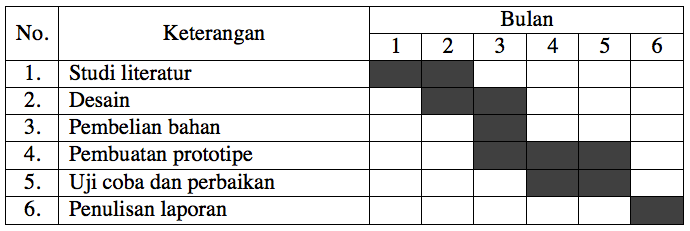
\includegraphics[width=13cm]{gambar/timeline}
\end{figure}

%-----------------------------------------------------------------
%Disini akhir masukan Bab
%-----------------------------------------------------------------

%-----------------------------------------------------------------
%Disini awal masukan untuk Daftar Pustaka
%-----------------------------------------------------------------
%%\nocite{Abel2010,Guerbas201350}
%%\bibliography{research-plan}
%%\bibliographystyle{plainnat}
\begin{thebibliography}{9}

\bibitem[satu(2013)]{satu01}
Winoto, Ardi. Mikrokontroler AVR ATmega8/16/32/8535 dan
Pemrogramannya dengan Bahasa C pada WinAVR. Informatika,
Bandung.2008. 

\bibitem[dua(2013)]{dua02}
Harara, Era, sistem pendeteksi kebocoran dan pengamanan dini
pada kompor Liquid Petrolium Gas (LPG) berbasis (Field
Programmable Gate Arrays) FPGA, STIKOM-Surabaya, 2007. 

\bibitem[dua(2013)]{tiga03}
Heryanto, Ary. Adi, Wisnu, 2008, Pemrograman Bahasa C untuk
Mikrokontroler ATmega8535, Andi, Yogyakarta.



\end{thebibliography}
\addcontentsline{toc}{chapter}{DAFTAR PUSTAKA}
%-----------------------------------------------------------------
%Disini akhir masukan Daftar Pustaka
%-----------------------------------------------------------------

\end{document}